\section{Programación del NIOS II \label{sec:s1}}

\begin{center}
	\begin{minipage}{12cm}
		\begin{tcolorbox}[title=Actividad 1]
			Basado en el sistema creado en la práctica 6, crear un programa que mande valores al puerto paralelo (PIO) de 8 bits, cada 1 segundo. Investigar la función para escribir en el puerto y la función para crear un retardo.
		\end{tcolorbox}	
	\end{minipage}
\end{center}



Siguiendo los pasos indicados en la presentación, se utiliza la herramienta \textit{Platform Designer} para crear el procesador NIOS II. Como se observa en la \autoref{fig:PlatformDesigner}, a los contenidos del sistema se le agrega un PIO, con el objetivo de observar la salida en hardware. Al momento de generar el procesador, se crea una carpeta en la que se halla el NIOS II (ver \autoref{fig:nios_path}).

La visualización RTL, del procesador NIOS II, se muestra en la \autoref{fig:nios_rtl1}. Ahora bien, realizando un acercamiento al módulo (ver \autoref{fig:nios_rtl2}), se observa que dentro del procesador se tienen los contenidos agregados en el \textit{Platform Designer}, como el módulo JTAG y el PIO.

En los Anexos se localiza la descripción del procesador NIOS II, que no es más que la instanciación del procesador en un proyecto previamente generado. 

\begin{figure}[ht]
	\centering
	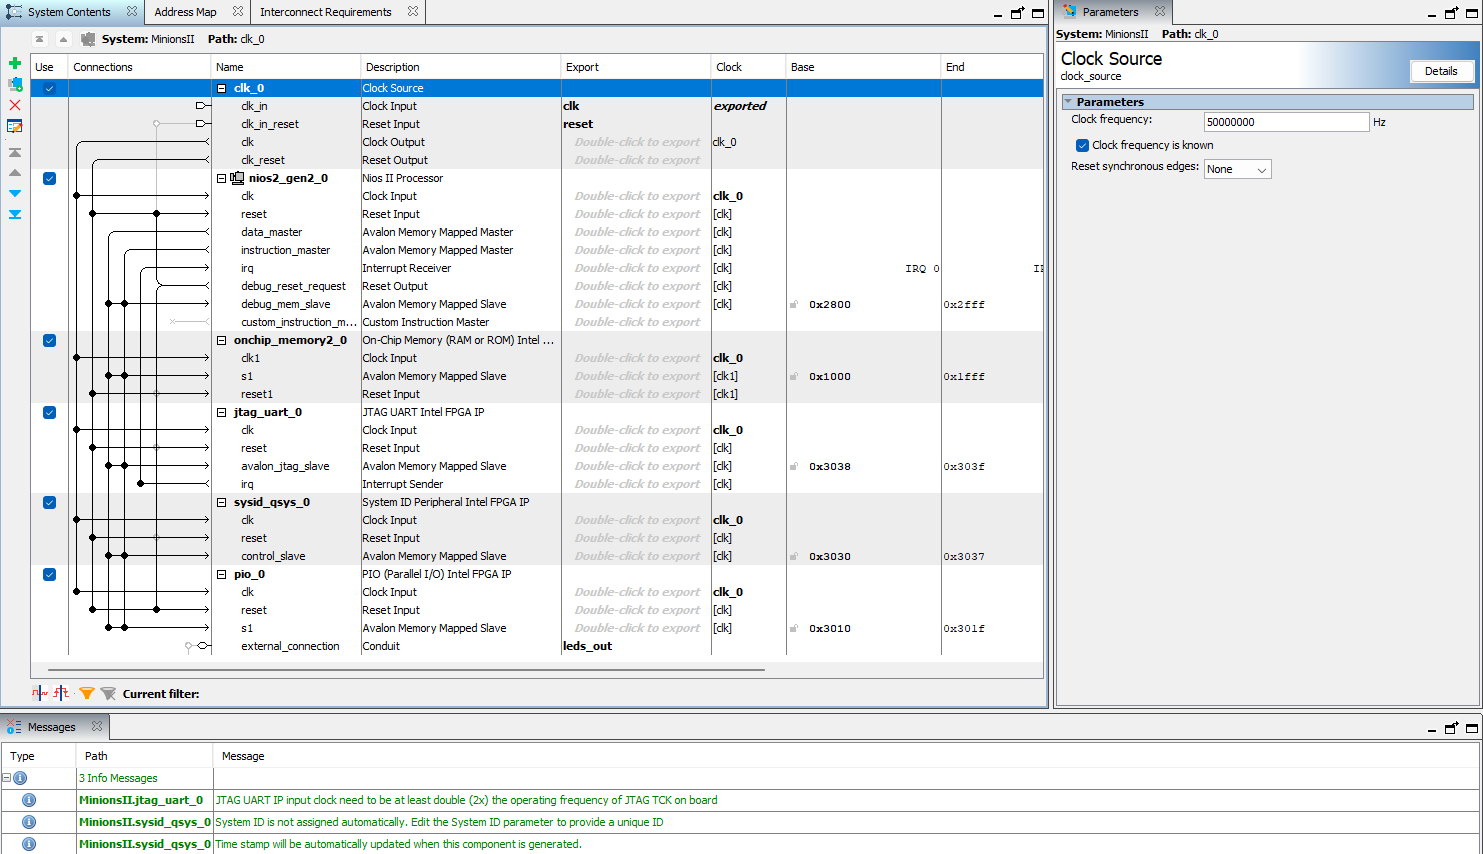
\includegraphics[scale=0.4]{PlatformDesigner.png}
	\caption{Vista del NIOS II desde el \textit{Platform Designer}. Se muestran todos los contenidos agregados al procesador. \label{fig:PlatformDesigner}}
\end{figure}

\begin{figure}[ht]
	\centering
	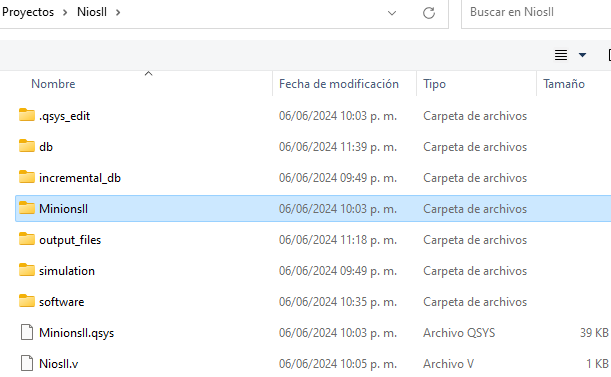
\includegraphics[scale=0.9]{NIOS_Path.png}
	\caption{Generación de la carpeta en donde se almacena al procesador NIOS II. \label{fig:nios_path}}
\end{figure}

\begin{figure}[ht]
	\centering
	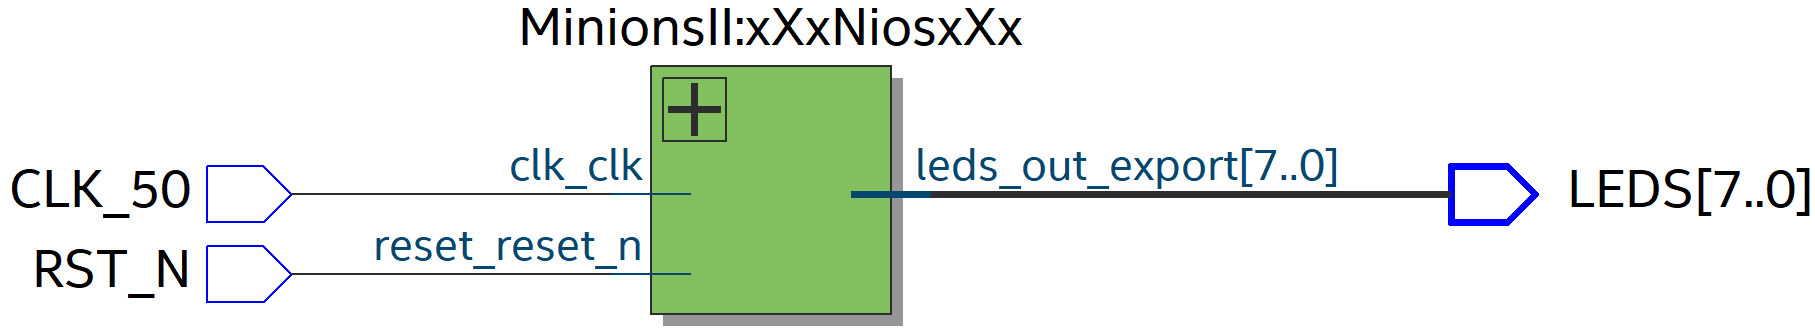
\includegraphics[scale=0.35]{NIOS_RTL1.png}
	\caption{Diagrama RTL del procesador NIOS II. \label{fig:nios_rtl1}}
\end{figure}

\begin{figure}[ht]
	\centering
	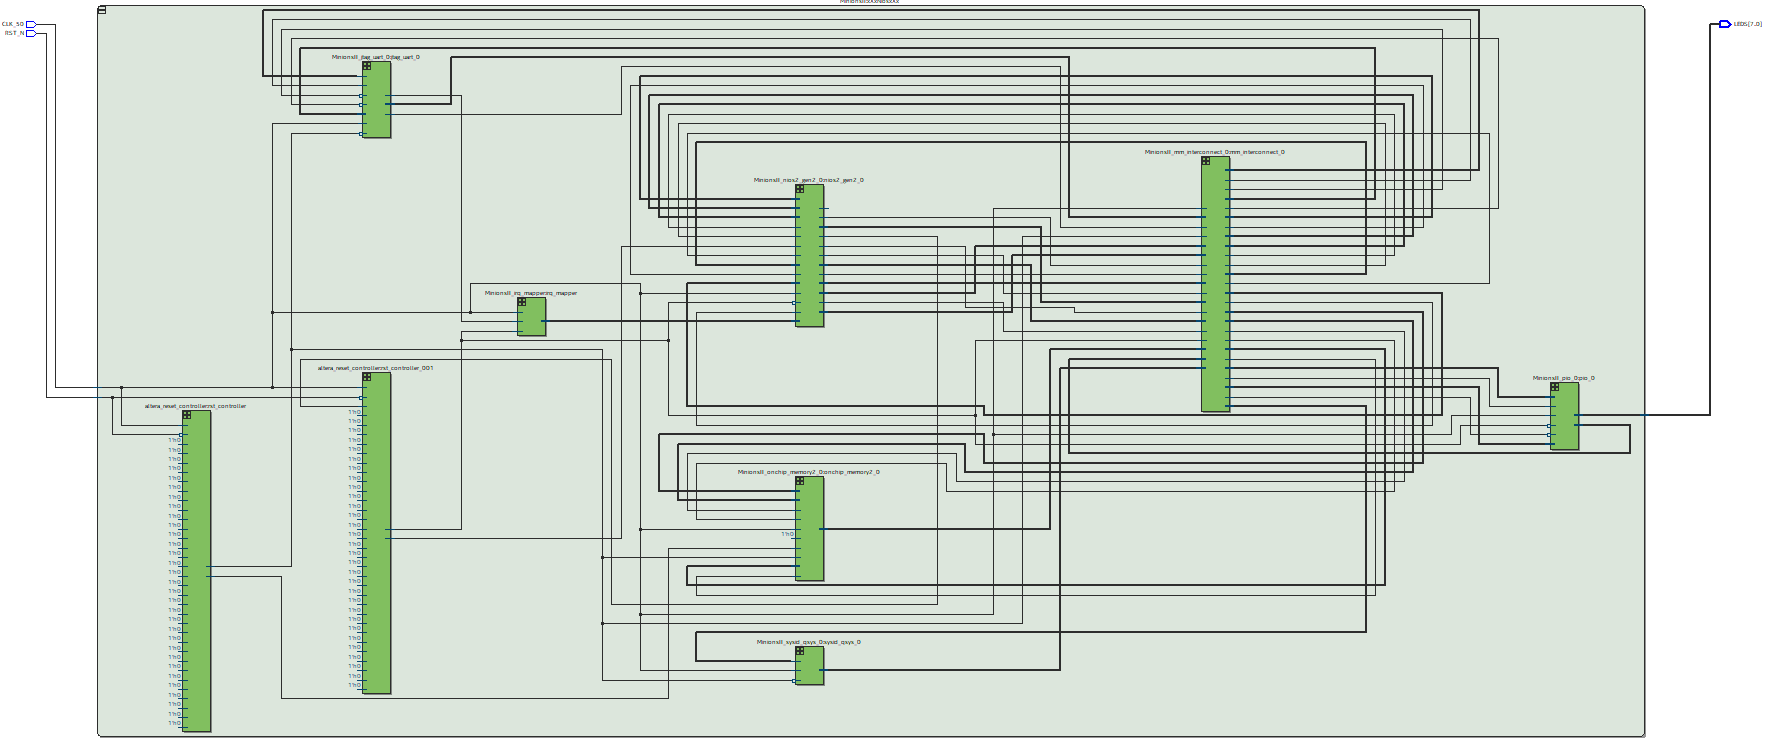
\includegraphics[scale=0.36]{NIOS_RTL2.png}
	\caption{Diagrama RTL del procesador NIOS II (acercamiento). \label{fig:nios_rtl2}}
\end{figure}